% Author: Izaak Neutelings (November 2021)
\documentclass[border=3pt,tikz]{standalone}
\usepackage{amsmath}
\tikzset{>=latex}
\usetikzlibrary{arrows.meta}
\usetikzlibrary{angles,quotes} % for pic

\colorlet{myorange}{orange!95!black}
\colorlet{mydarkblue}{blue!20!black}


\begin{document}


% HIGH PT TAU: collimated pions
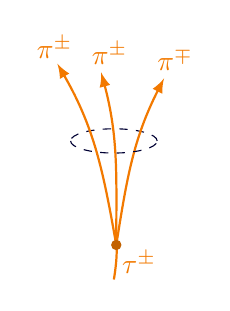
\begin{tikzpicture}[scale=2.2]
  
  \coordinate (O) at (0,0);
  \coordinate (T) at (86:0.2);
  \coordinate (C) at (90:0.8); % ellipse center
  \def\rx{0.25} % horizontal radius of ellipse
  \def\ry{0.07} % vertical radius of ellipse
  
  % TAU
  \draw[thick,myorange]
    (O) to[out=80,in=-80,looseness=0.6] (T);
  \path (O) -- (T) node[myorange,pos=0.5,right=-1] {$\tau^\pm$};
  
  % PIONS
  \draw[dashed,mydarkblue]
    (C)++(\rx,0) arc(0:180:{\rx} and \ry);
  \draw[->,myorange,thick]
    (T) to[out=100,in=-60] ++(108:1.1) node[left=1,above=-2] {$\pi^\pm$};
  \draw[->,myorange,thick]
    (T) to[out=90,in=-75] ++(95:1.0) node[right=3,above=-1] {$\pi^\pm$};
  \draw[->,myorange,thick]
    (T) to[out=81,in=-117] ++(74:1.0) node[right=4,above=-1] {$\pi^\mp$};
  \fill[myorange!80!black] (T) circle (0.03);
  \draw[dashed,mydarkblue]
    (C)++(-\rx,0) arc(180:360:{\rx} and \ry);
  
\end{tikzpicture}


\end{document}